\documentclass[11pt]{article}
\usepackage[a4paper,margin=2.3cm]{geometry}
\usepackage{booktabs,graphicx,tabularx,array,caption,amsmath,xcolor,float,placeins}
\usepackage[hidelinks]{hyperref}
\usepackage{microtype}
\captionsetup{font=small,labelfont=bf,skip=4pt}
\newcolumntype{L}{>{\raggedright\arraybackslash}X}
\newcommand{\tabnote}[1]{\par\vspace{3pt}\footnotesize\emph{Notes:} #1\normalsize}
\newcommand{\nDrawn}{1485}\newcommand{\nFiled}{416}\newcommand{\nReceipt}{394}\newcommand{\nDated}{242}\newcommand{\nResp}{9}\newcommand{\asof}{24 September 2026}
\newcommand{\attrN}{1000}\newcommand{\attrB}{-0.4}\newcommand{\attrSE}{2.0}\newcommand{\attrP}{0.84}\newcommand{\attrRI}{0.64}\newcommand{\attrStrata}{115}
\newcommand{\balPtier}{0.00}\newcommand{\balPra}{1.00}
\newcommand{\kmSeven}{2.3}\newcommand{\riskSeven}{211}\newcommand{\kmFourteen}{3.2}\newcommand{\riskFourteen}{166}\newcommand{\kmTwentyOne}{4.5}\newcommand{\riskTwentyOne}{135}\newcommand{\kmTwentyEight}{4.5}\newcommand{\riskTwentyEight}{19}

\title{RTI audit, wave 1: filings and early responses\\[2pt]\large Preliminary report consistent with the pre-analysis plan}
\author{Amar Priyadarshi\thanks{Prepared with Gaurav Sood in view. Data as of \asof. Every table is generated by \texttt{reports/report1\_filings/analysis.py} in the \texttt{rti-responses} repository from the frozen assignment files, the RAs' filing sheets and receipts, and the coded responses.}}
\date{\asof}
\begin{document}
\maketitle

\section*{Scope and discipline}
This report covers what the pre-analysis plan (design document v0.1, Sections 2 and 5) allows before outcomes are observed: the drawn and realised samples, balance, filing-stage access costs, exposure time, and the early-response hazard. As of \asof\ no filed application has reached its 30-day statutory deadline, so response incidence is unobserved for the entire sample. Treatment arms appear only where the plan treats them as design or pre-treatment quantities: the design table, the filing-attrition test, and balance. No outcome is tabulated by arm; that begins once the plan is posted and the day-30 horizon has passed for the Tamil Nadu batch.

\section{Drawn samples}
\begin{table}[H]\centering\small
\caption{Drawn samples by state (frozen assignment files)}
\begin{tabularx}{\textwidth}{lrrLrr}\toprule
State & $N$ & Plain / Legal & Tiers & RA1/RA2/RA3/RA4 & Strata \\\midrule
\csname @@input\endcsname tab_design.tex 
\bottomrule\end{tabularx}
\tabnote{Batches: Tamil Nadu \texttt{b2026q3\_02} (seed 20260817), Telangana \texttt{tg2026q3\_02} (20260903), Karnataka \texttt{ka2026q3\_01} (20260907), Delhi and Maharashtra \texttt{dm2026q3\_01} (20260908). Tamil Nadu is stratified by department $\times$ tier from the crawled 17,417-office universe; the other states are drawn from portal rosters stratified by department group. Salience is a seeded 70/30 draw within each batch; RA assignment is round-robin within strata.}
\end{table}

\section{Realised filing and attrition}
\begin{table}[H]\centering\small
\caption{Filing progress by state and arm, as of \asof}
\begin{tabular}{lrrrrrr}\toprule
State & Drawn & Filed & Filed (\%) & Plain (\%) & Legal (\%) & Difference (pp) \\\midrule
\csname @@input\endcsname tab_filing.tex 
\bottomrule\end{tabular}
\tabnote{``Filed'' means a portal receipt is uploaded to the shared drive or the RA's sheet records a registration number or filing date (\nFiled\ applications, of which \nReceipt\ have receipts). Filing is in progress, so the filed share is a throughput measure, not attrition; the arm difference is the pre-treatment check that RAs did not file selectively by letter type. Tamil Nadu, the fully stratified batch: a linear probability model of filed-by-\asof\ on the legal-salience indicator with \attrStrata\ department $\times$ tier stratum fixed effects gives \attrB\ pp (HC1 s.e. \attrSE), $p = \attrP$; randomisation inference within strata (2,000 permutations) gives $p = \attrRI$.}
\end{table}

\begin{figure}[H]\centering
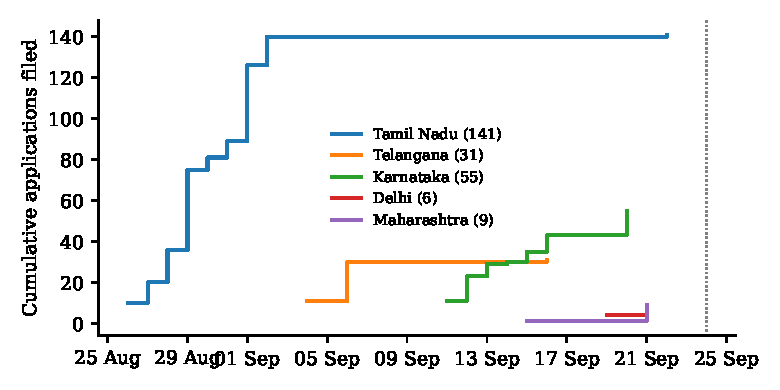
\includegraphics{fig_timeline.pdf}
\caption{Cumulative filings by state}
\tabnote{Applications with a recorded filing date (\nDated\ of \nFiled). Telangana dates are under-recorded in the RA sheets (31 of 187); receipt OCR will fill them.}
\end{figure}

\begin{table}[H]\centering\small
\caption{Balance of the filed Tamil Nadu sample across arms}
\begin{tabular}{lrrrr}\toprule
 & Filed & Plain & Legal & Legal (\%) \\\midrule
\csname @@input\endcsname tab_balance.tex 
\bottomrule\end{tabular}
\tabnote{Chi-square tests of independence between arm and tier ($p = \balPtier$) and between arm and research assistant ($p = \balPra$). The draw is balanced by construction; imbalance in the filed subset reflects the order in which RAs have worked through their lists and will close as filing completes. It is reported so that any early-window comparison would be read with it.}
\end{table}

\section{Filing-stage access costs}
\begin{table}[H]\centering\scriptsize
\caption{What an online filer faces, by state portal}
\begin{tabularx}{\textwidth}{lLLcccLLL}\toprule
State & Portal & Universe & VPN & OTP & CAPTCHAs & Fee channel & Text limit & Identity demand \\\midrule
\csname @@input\endcsname tab_access.tex 
\bottomrule\end{tabularx}
\tabnote{From the RAs' screen recordings, portal field inventories and filing notes. ``VPN'' means the portal is unreachable from outside India. Rajasthan was dropped from the frame at this stage: the portal requires an identity-document number and scan and a Rajasthan postal address, which is itself a frame-level finding. Maharashtra's 150-word cap forced a condensed instrument (v4) for its 33 assignments; Delhi keeps v3. RA minutes per filing from the hours sheet will be added in the next version.}
\end{table}

\section{Exposure and the early-response hazard}
\begin{table}[H]\centering\small
\caption{Exposure of filed applications, as of \asof}
\begin{tabular}{lrrrlrrr}\toprule
State & Filed & Receipts & Dated & Filing window & Median days & Max days & Past day 30 \\\midrule
\csname @@input\endcsname tab_exposure.tex 
\bottomrule\end{tabular}
\tabnote{Days from the portal's date of filing to \asof. No application has reached the statutory deadline; the earliest Tamil Nadu filings (26 August) reach day 30 on 25 September, Karnataka's on 12 October, Telangana's from 4 October.}
\end{table}

\begin{figure}[H]\centering
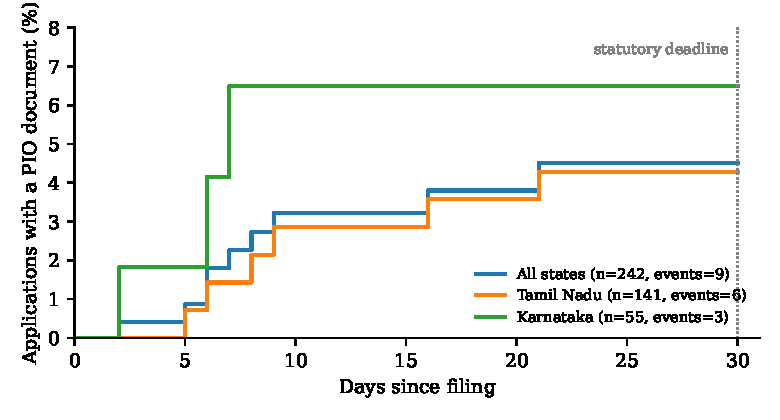
\includegraphics{fig_km.pdf}
\caption{Cumulative incidence of a PIO document by days since filing (Kaplan--Meier, censored at \asof)}
\tabnote{Event = any PIO document dated $t$ days after filing (portal reply, letter, transfer, fee demand, or return). Applications without an event are censored at their exposure. Estimates: \kmSeven\% by day 7 (\riskSeven\ at risk), \kmFourteen\% by day 14 (\riskFourteen), \kmTwentyOne\% by day 21 (\riskTwentyOne), \kmTwentyEight\% by day 28 (\riskTwentyEight\ at risk). The plan's primary display is Kaplan--Meier by stratum with censoring at 90 and 180 days; this is the same object truncated at day 30 and pooled because there are \nResp\ events. Postal replies are dated by the PIO's letter, which precedes receipt.}
\end{figure}

\section{The first responses}
\begin{table}[H]\centering\scriptsize
\caption{The \nResp\ responses received, coded on the plan's ladder (SI~C), without arm}
\begin{tabularx}{\textwidth}{lLrrrlLLr}\toprule
ID & Authority & Filed & Replied & Days & Via & Disposition & Granularity & Fee \\\midrule
\csname @@input\endcsname tab_responses.tex 
\bottomrule\end{tabularx}
\tabnote{Single-coder first pass, to be replaced by double coding. ``Denied (deflection)'' covers a refusal without an exemption clause that points elsewhere (a portal return; ``file a separate application''; ``see cic.gov.in''). ``Fee pending'' means the register was offered on payment at the lawful Rs~2 per page. Granularity follows the letter's ladder: A = one row per RTI application in the office's register; B = monthly or category counts; C = period totals. Only one of the nine honoured the request for scanned supply by email.}
\end{table}

\section*{What comes next}
Day-30 outcomes for Tamil Nadu accumulate from 25 September; the first-results memo at day 45 (mid-October) reports the plan's primary display by stratum and the day-30 incidence, with the legal-salience contrast only after the plan is posted. Two data tasks precede it: complete the filing dates from receipt OCR (Telangana), and move response intake to the event log so that receipt dates, not dispatch dates, drive the survival clock.
\end{document}
